\documentclass[1p]{elsarticle_modified}
%\bibliographystyle{elsarticle-num}

%\usepackage[colorlinks]{hyperref}
%\usepackage{abbrmath_seonhwa} %\Abb, \Ascr, \Acal ,\Abf, \Afrak
\usepackage{amsfonts}
\usepackage{amssymb}
\usepackage{amsmath}
\usepackage{amsthm}
\usepackage{scalefnt}
\usepackage{amsbsy}
\usepackage{kotex}
\usepackage{caption}
\usepackage{subfig}
\usepackage{color}
\usepackage{graphicx}
\usepackage{xcolor} %% white, black, red, green, blue, cyan, magenta, yellow
\usepackage{float}
\usepackage{setspace}
\usepackage{hyperref}

\usepackage{tikz}
\usetikzlibrary{arrows}

\usepackage{multirow}
\usepackage{array} % fixed length table
\usepackage{hhline}

%%%%%%%%%%%%%%%%%%%%%
\makeatletter
\renewcommand*\env@matrix[1][\arraystretch]{%
	\edef\arraystretch{#1}%
	\hskip -\arraycolsep
	\let\@ifnextchar\new@ifnextchar
	\array{*\c@MaxMatrixCols c}}
\makeatother %https://tex.stackexchange.com/questions/14071/how-can-i-increase-the-line-spacing-in-a-matrix
%%%%%%%%%%%%%%%

\usepackage[normalem]{ulem}

\newcommand{\msout}[1]{\ifmmode\text{\sout{\ensuremath{#1}}}\else\sout{#1}\fi}
%SOURCE: \msout is \stkout macro in https://tex.stackexchange.com/questions/20609/strikeout-in-math-mode

\newcommand{\cancel}[1]{
	\ifmmode
	{\color{red}\msout{#1}}
	\else
	{\color{red}\sout{#1}}
	\fi
}

\newcommand{\add}[1]{
	{\color{blue}\uwave{#1}}
}

\newcommand{\replace}[2]{
	\ifmmode
	{\color{red}\msout{#1}}{\color{blue}\uwave{#2}}
	\else
	{\color{red}\sout{#1}}{\color{blue}\uwave{#2}}
	\fi
}

\newcommand{\Sol}{\mathcal{S}} %segment
\newcommand{\D}{D} %diagram
\newcommand{\A}{\mathcal{A}} %arc


%%%%%%%%%%%%%%%%%%%%%%%%%%%%%5 test

\def\sl{\operatorname{\textup{SL}}(2,\Cbb)}
\def\psl{\operatorname{\textup{PSL}}(2,\Cbb)}
\def\quan{\mkern 1mu \triangleright \mkern 1mu}

\theoremstyle{definition}
\newtheorem{thm}{Theorem}[section]
\newtheorem{prop}[thm]{Proposition}
\newtheorem{lem}[thm]{Lemma}
\newtheorem{ques}[thm]{Question}
\newtheorem{cor}[thm]{Corollary}
\newtheorem{defn}[thm]{Definition}
\newtheorem{exam}[thm]{Example}
\newtheorem{rmk}[thm]{Remark}
\newtheorem{alg}[thm]{Algorithm}

\newcommand{\I}{\sqrt{-1}}
\begin{document}

%\begin{frontmatter}
%
%\title{Boundary parabolic representations of knots up to 8 crossings}
%
%%% Group authors per affiliation:
%\author{Yunhi Cho} 
%\address{Department of Mathematics, University of Seoul, Seoul, Korea}
%\ead{yhcho@uos.ac.kr}
%
%
%\author{Seonhwa Kim} %\fnref{s_kim}}
%\address{Center for Geometry and Physics, Institute for Basic Science, Pohang, 37673, Korea}
%\ead{ryeona17@ibs.re.kr}
%
%\author{Hyuk Kim}
%\address{Department of Mathematical Sciences, Seoul National University, Seoul 08826, Korea}
%\ead{hyukkim@snu.ac.kr}
%
%\author{Seokbeom Yoon}
%\address{Department of Mathematical Sciences, Seoul National University, Seoul, 08826,  Korea}
%\ead{sbyoon15@snu.ac.kr}
%
%\begin{abstract}
%We find all boundary parabolic representation of knots up to 8 crossings.
%
%\end{abstract}
%\begin{keyword}
%    \MSC[2010] 57M25 
%\end{keyword}
%
%\end{frontmatter}

%\linenumbers
%\tableofcontents
%
\newcommand\colored[1]{\textcolor{white}{\rule[-0.35ex]{0.8em}{1.4ex}}\kern-0.8em\color{red} #1}%
%\newcommand\colored[1]{\textcolor{white}{ #1}\kern-2.17ex	\textcolor{white}{ #1}\kern-1.81ex	\textcolor{white}{ #1}\kern-2.15ex\color{red}#1	}

{\Large $\underline{12a_{0210}~(K12a_{0210})}$}

\setlength{\tabcolsep}{10pt}
\renewcommand{\arraystretch}{1.6}
\vspace{1cm}\begin{tabular}{m{100pt}>{\centering\arraybackslash}m{274pt}}
\multirow{5}{120pt}{
	\centering
	\includegraphics[width=112pt]{../../../GIT/diagram.site/Diagrams/png/1011_12a_0210.png}\\
\ \ \ A knot diagram\footnotemark}&
\allowdisplaybreaks
\textbf{Linearized knot diagam} \\
\cline{2-2}
 &
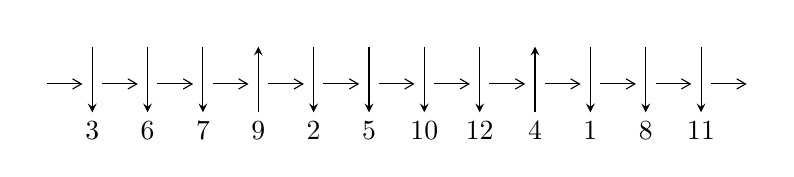
\begin{tikzpicture}[x=20pt, y=17pt]
	% nodes
	\node (C0) at (0, 0) {};
	\node (C1) at (1, 0) {};
	\node (C1U) at (1, +1) {};
	\node (C1D) at (1, -1) {3};

	\node (C2) at (2, 0) {};
	\node (C2U) at (2, +1) {};
	\node (C2D) at (2, -1) {6};

	\node (C3) at (3, 0) {};
	\node (C3U) at (3, +1) {};
	\node (C3D) at (3, -1) {7};

	\node (C4) at (4, 0) {};
	\node (C4U) at (4, +1) {};
	\node (C4D) at (4, -1) {9};

	\node (C5) at (5, 0) {};
	\node (C5U) at (5, +1) {};
	\node (C5D) at (5, -1) {2};

	\node (C6) at (6, 0) {};
	\node (C6U) at (6, +1) {};
	\node (C6D) at (6, -1) {5};

	\node (C7) at (7, 0) {};
	\node (C7U) at (7, +1) {};
	\node (C7D) at (7, -1) {10};

	\node (C8) at (8, 0) {};
	\node (C8U) at (8, +1) {};
	\node (C8D) at (8, -1) {12};

	\node (C9) at (9, 0) {};
	\node (C9U) at (9, +1) {};
	\node (C9D) at (9, -1) {4};

	\node (C10) at (10, 0) {};
	\node (C10U) at (10, +1) {};
	\node (C10D) at (10, -1) {1};

	\node (C11) at (11, 0) {};
	\node (C11U) at (11, +1) {};
	\node (C11D) at (11, -1) {8};

	\node (C12) at (12, 0) {};
	\node (C12U) at (12, +1) {};
	\node (C12D) at (12, -1) {11};
	\node (C13) at (13, 0) {};

	% arrows
	\draw[->,>={angle 60}]
	(C0) edge (C1) (C1) edge (C2) (C2) edge (C3) (C3) edge (C4) (C4) edge (C5) (C5) edge (C6) (C6) edge (C7) (C7) edge (C8) (C8) edge (C9) (C9) edge (C10) (C10) edge (C11) (C11) edge (C12) (C12) edge (C13) ;	\draw[->,>=stealth]
	(C1U) edge (C1D) (C2U) edge (C2D) (C3U) edge (C3D) (C4D) edge (C4U) (C5U) edge (C5D) (C6U) edge (C6D) (C7U) edge (C7D) (C8U) edge (C8D) (C9D) edge (C9U) (C10U) edge (C10D) (C11U) edge (C11D) (C12U) edge (C12D) ;
	\end{tikzpicture} \\
\hhline{~~} \\& 
\textbf{Solving Sequence} \\ \cline{2-2} 
 &
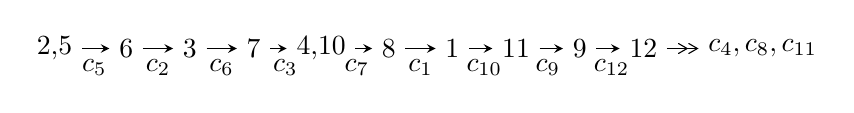
\begin{tikzpicture}[x=23pt, y=7pt]
	% node
	\node (A0) at (-1/8, 0) {2,5};
	\node (A1) at (1, 0) {6};
	\node (A2) at (2, 0) {3};
	\node (A3) at (3, 0) {7};
	\node (A4) at (65/16, 0) {4,10};
	\node (A5) at (41/8, 0) {8};
	\node (A6) at (49/8, 0) {1};
	\node (A7) at (57/8, 0) {11};
	\node (A8) at (65/8, 0) {9};
	\node (A9) at (73/8, 0) {12};
	\node (C1) at (1/2, -1) {$c_{5}$};
	\node (C2) at (3/2, -1) {$c_{2}$};
	\node (C3) at (5/2, -1) {$c_{6}$};
	\node (C4) at (7/2, -1) {$c_{3}$};
	\node (C5) at (37/8, -1) {$c_{7}$};
	\node (C6) at (45/8, -1) {$c_{1}$};
	\node (C7) at (53/8, -1) {$c_{10}$};
	\node (C8) at (61/8, -1) {$c_{9}$};
	\node (C9) at (69/8, -1) {$c_{12}$};
	\node (A10) at (11, 0) {$c_{4},c_{8},c_{11}$};

	% edge
	\draw[->,>=stealth]	
	(A0) edge (A1) (A1) edge (A2) (A2) edge (A3) (A3) edge (A4) (A4) edge (A5) (A5) edge (A6) (A6) edge (A7) (A7) edge (A8) (A8) edge (A9) ;
	\draw[->>,>={angle 60}]	
	(A9) edge (A10);
\end{tikzpicture} \\ 

\end{tabular} \\

\footnotetext{
The image of knot diagram is generated by the software ``\textbf{Draw programme}" developed by Andrew Bartholomew(\url{http://www.layer8.co.uk/maths/draw/index.htm\#Running-draw}), where we modified some parts for our purpose(\url{https://github.com/CATsTAILs/LinksPainter}).
}\phantom \\ \newline 
\centering \textbf{Ideals for irreducible components\footnotemark of $X_{\text{par}}$} 
 
\begin{align*}
I^u_{1}&=\langle 
- u^{17}+3 u^{15}+u^{14}-7 u^{13}-2 u^{12}+9 u^{11}+5 u^{10}-10 u^9-5 u^8+7 u^7+6 u^6-5 u^5-3 u^4+u^3+2 u^2+b,\\
\phantom{I^u_{1}}&\phantom{= \langle  }- u^{15}+2 u^{13}+u^{12}-4 u^{11}- u^{10}+3 u^9+3 u^8-3 u^7- u^6+u^5+2 u^4- u^3+a- u,\;u^{18}-3 u^{16}+\cdots+2 u+1\rangle \\
I^u_{2}&=\langle 
3 u^{83}+6 u^{82}+\cdots+b-1,\;7 u^{83}+10 u^{82}+\cdots+2 a-11,\;u^{84}+3 u^{83}+\cdots+2 u-1\rangle \\
I^u_{3}&=\langle 
b,\;a+1,\;u^3- u^2+1\rangle \\
I^u_{4}&=\langle 
b,\;a^2- a u+2 u^2-3 u+2,\;u^3- u^2+1\rangle \\
I^u_{5}&=\langle 
b-2,\;a-1,\;u+1\rangle \\
\\
\end{align*}
\raggedright * 5 irreducible components of $\dim_{\mathbb{C}}=0$, with total 112 representations.\\
\footnotetext{All coefficients of polynomials are rational numbers. But the coefficients are sometimes approximated in decimal forms when there is not enough margin.}
\newpage
\renewcommand{\arraystretch}{1}
\centering \section*{I. $I^u_{1}= \langle - u^{17}+3 u^{15}+\cdots+2 u^2+b,\;- u^{15}+2 u^{13}+\cdots+a- u,\;u^{18}-3 u^{16}+\cdots+2 u+1 \rangle$}
\flushleft \textbf{(i) Arc colorings}\\
\begin{tabular}{m{7pt} m{180pt} m{7pt} m{180pt} }
\flushright $a_{2}=$&$\begin{pmatrix}0\\u\end{pmatrix}$ \\
\flushright $a_{5}=$&$\begin{pmatrix}1\\0\end{pmatrix}$ \\
\flushright $a_{6}=$&$\begin{pmatrix}1\\u^2\end{pmatrix}$ \\
\flushright $a_{3}=$&$\begin{pmatrix}- u\\- u^3+u\end{pmatrix}$ \\
\flushright $a_{7}=$&$\begin{pmatrix}- u^2+1\\u^2\end{pmatrix}$ \\
\flushright $a_{4}=$&$\begin{pmatrix}u^7-2 u^5+2 u^3-2 u\\- u^7+u^5-2 u^3+u\end{pmatrix}$ \\
\flushright $a_{10}=$&$\begin{pmatrix}u^{15}-2 u^{13}- u^{12}+4 u^{11}+u^{10}-3 u^9-3 u^8+3 u^7+u^6- u^5-2 u^4+u^3+u\\u^{17}-3 u^{15}+\cdots- u^3-2 u^2\end{pmatrix}$ \\
\flushright $a_{8}=$&$\begin{pmatrix}- u^{16}+3 u^{14}+\cdots- u^2+1\\u^{16}-2 u^{14}+\cdots- u^4+2 u^2\end{pmatrix}$ \\
\flushright $a_{1}=$&$\begin{pmatrix}u^3\\u^5- u^3+u\end{pmatrix}$ \\
\flushright $a_{11}=$&$\begin{pmatrix}u^{15}-2 u^{13}- u^{12}+4 u^{11}+u^{10}-3 u^9-3 u^8+3 u^7+u^6-2 u^4+u^3+u\\u^{17}-3 u^{15}+\cdots+3 u^4-2 u^2\end{pmatrix}$ \\
\flushright $a_{9}=$&$\begin{pmatrix}u^{14}-3 u^{12}+\cdots+2 u^2+2 u\\- u^{14}+2 u^{12}+u^{11}-5 u^{10}- u^9+5 u^8+3 u^7-6 u^6- u^5+3 u^4+2 u^3-2 u^2\end{pmatrix}$ \\
\flushright $a_{12}=$&$\begin{pmatrix}u^{17}-2 u^{15}- u^{14}+4 u^{13}+u^{12}-3 u^{11}-3 u^{10}+3 u^9+u^8-2 u^6+u^5+2 u^3\\- u^{15}+3 u^{13}+\cdots-2 u^3-2 u^2\end{pmatrix}$\\&\end{tabular}
\flushleft \textbf{(ii) Obstruction class $= -1$}\\~\\
\flushleft \textbf{(iii) Cusp Shapes $= -2 u^{17}+4 u^{16}+8 u^{15}-10 u^{14}-24 u^{13}+26 u^{12}+42 u^{11}-30 u^{10}-66 u^9+34 u^8+66 u^7-16 u^6-66 u^5+8 u^4+32 u^3+8 u^2-16 u-14$}\\~\\
\newpage\renewcommand{\arraystretch}{1}
\flushleft \textbf{(iv) u-Polynomials at the component}\newline \\
\begin{tabular}{m{50pt}|m{274pt}}
Crossings & \hspace{64pt}u-Polynomials at each crossing \\
\hline $$\begin{aligned}c_{1},c_{6},c_{10}\\c_{12}\end{aligned}$$&$\begin{aligned}
&u^{18}+6 u^{17}+\cdots+2 u+1
\end{aligned}$\\
\hline $$\begin{aligned}c_{2},c_{5},c_{8}\\c_{11}\end{aligned}$$&$\begin{aligned}
&u^{18}-3 u^{16}+\cdots+2 u+1
\end{aligned}$\\
\hline $$\begin{aligned}c_{3},c_{7}\end{aligned}$$&$\begin{aligned}
&u^{18}-2 u^{17}+\cdots+4 u+1
\end{aligned}$\\
\hline $$\begin{aligned}c_{4},c_{9}\end{aligned}$$&$\begin{aligned}
&u^{18}-6 u^{17}+\cdots-24 u+8
\end{aligned}$\\
\hline
\end{tabular}\\~\\
\newpage\renewcommand{\arraystretch}{1}
\flushleft \textbf{(v) Riley Polynomials at the component}\newline \\
\begin{tabular}{m{50pt}|m{274pt}}
Crossings & \hspace{64pt}Riley Polynomials at each crossing \\
\hline $$\begin{aligned}c_{1},c_{6},c_{10}\\c_{12}\end{aligned}$$&$\begin{aligned}
&y^{18}+14 y^{17}+\cdots+22 y+1
\end{aligned}$\\
\hline $$\begin{aligned}c_{2},c_{5},c_{8}\\c_{11}\end{aligned}$$&$\begin{aligned}
&y^{18}-6 y^{17}+\cdots-2 y+1
\end{aligned}$\\
\hline $$\begin{aligned}c_{3},c_{7}\end{aligned}$$&$\begin{aligned}
&y^{18}-10 y^{17}+\cdots-2 y+1
\end{aligned}$\\
\hline $$\begin{aligned}c_{4},c_{9}\end{aligned}$$&$\begin{aligned}
&y^{18}+8 y^{17}+\cdots+256 y+64
\end{aligned}$\\
\hline
\end{tabular}\\~\\
\newpage\flushleft \textbf{(vi) Complex Volumes and Cusp Shapes}
$$\begin{array}{c|c|c}  
\text{Solutions to }I^u_{1}& \I (\text{vol} + \sqrt{-1}CS) & \text{Cusp shape}\\
 \hline 
\begin{aligned}
u &= \phantom{-}0.852988 + 0.599070 I \\
a &= \phantom{-}1.86967 + 1.04403 I \\
b &= -1.54451 + 0.51046 I\end{aligned}
 & \phantom{-}2.34312 - 4.73471 I & -7.07668 + 6.82584 I \\ \hline\begin{aligned}
u &= \phantom{-}0.852988 - 0.599070 I \\
a &= \phantom{-}1.86967 - 1.04403 I \\
b &= -1.54451 - 0.51046 I\end{aligned}
 & \phantom{-}2.34312 + 4.73471 I & -7.07668 - 6.82584 I \\ \hline\begin{aligned}
u &= \phantom{-}0.713575 + 0.772455 I \\
a &= -1.68389 + 1.91803 I \\
b &= \phantom{-}0.92095 - 1.86302 I\end{aligned}
 & \phantom{-}5.76795 - 0.42490 I & -2.62552 + 1.94246 I \\ \hline\begin{aligned}
u &= \phantom{-}0.713575 - 0.772455 I \\
a &= -1.68389 - 1.91803 I \\
b &= \phantom{-}0.92095 + 1.86302 I\end{aligned}
 & \phantom{-}5.76795 + 0.42490 I & -2.62552 - 1.94246 I \\ \hline\begin{aligned}
u &= -0.680242 + 0.830816 I \\
a &= \phantom{-}1.80309 + 1.05417 I \\
b &= -1.63673 - 1.25883 I\end{aligned}
 & \phantom{-}3.89996 - 5.56871 I & -4.31829 + 2.06139 I \\ \hline\begin{aligned}
u &= -0.680242 - 0.830816 I \\
a &= \phantom{-}1.80309 - 1.05417 I \\
b &= -1.63673 + 1.25883 I\end{aligned}
 & \phantom{-}3.89996 + 5.56871 I & -4.31829 - 2.06139 I \\ \hline\begin{aligned}
u &= \phantom{-}1.088500 + 0.110069 I \\
a &= -0.751912 + 0.070278 I \\
b &= -1.65982 + 0.10721 I\end{aligned}
 & -9.12746 - 5.02050 I & -18.4222 + 4.8342 I \\ \hline\begin{aligned}
u &= \phantom{-}1.088500 - 0.110069 I \\
a &= -0.751912 - 0.070278 I \\
b &= -1.65982 - 0.10721 I\end{aligned}
 & -9.12746 + 5.02050 I & -18.4222 - 4.8342 I \\ \hline\begin{aligned}
u &= -1.012600 + 0.591290 I \\
a &= -0.91949 - 1.13440 I \\
b &= \phantom{-}0.066057 + 0.911088 I\end{aligned}
 & -3.35551 + 7.83027 I & -12.5543 - 7.9398 I \\ \hline\begin{aligned}
u &= -1.012600 - 0.591290 I \\
a &= -0.91949 + 1.13440 I \\
b &= \phantom{-}0.066057 - 0.911088 I\end{aligned}
 & -3.35551 - 7.83027 I & -12.5543 + 7.9398 I\\
 \hline 
 \end{array}$$\newpage$$\begin{array}{c|c|c}  
\text{Solutions to }I^u_{1}& \I (\text{vol} + \sqrt{-1}CS) & \text{Cusp shape}\\
 \hline 
\begin{aligned}
u &= \phantom{-}0.997184 + 0.703282 I \\
a &= \phantom{-}1.01150 - 3.14671 I \\
b &= \phantom{-}1.47517 + 2.11590 I\end{aligned}
 & \phantom{-}4.02002 - 10.78450 I & -6.41328 + 8.53348 I \\ \hline\begin{aligned}
u &= \phantom{-}0.997184 - 0.703282 I \\
a &= \phantom{-}1.01150 + 3.14671 I \\
b &= \phantom{-}1.47517 - 2.11590 I\end{aligned}
 & \phantom{-}4.02002 + 10.78450 I & -6.41328 - 8.53348 I \\ \hline\begin{aligned}
u &= -0.623040 + 0.431726 I \\
a &= -0.237344 + 0.890114 I \\
b &= \phantom{-}0.157083 + 0.325898 I\end{aligned}
 & -0.68211 + 1.26711 I & -9.25343 - 4.35410 I \\ \hline\begin{aligned}
u &= -0.623040 - 0.431726 I \\
a &= -0.237344 - 0.890114 I \\
b &= \phantom{-}0.157083 - 0.325898 I\end{aligned}
 & -0.68211 - 1.26711 I & -9.25343 + 4.35410 I \\ \hline\begin{aligned}
u &= -1.029700 + 0.727727 I \\
a &= -0.09346 - 2.99952 I \\
b &= -2.04495 + 1.32035 I\end{aligned}
 & \phantom{-}1.7668 + 17.2595 I & -7.77898 - 11.27344 I \\ \hline\begin{aligned}
u &= -1.029700 - 0.727727 I \\
a &= -0.09346 + 2.99952 I \\
b &= -2.04495 - 1.32035 I\end{aligned}
 & \phantom{-}1.7668 - 17.2595 I & -7.77898 + 11.27344 I \\ \hline\begin{aligned}
u &= -0.306671 + 0.477938 I \\
a &= \phantom{-}0.001829 + 0.467096 I \\
b &= -0.233244 + 0.353264 I\end{aligned}
 & -0.520477 + 1.222060 I & -5.55737 - 4.78188 I \\ \hline\begin{aligned}
u &= -0.306671 - 0.477938 I \\
a &= \phantom{-}0.001829 - 0.467096 I \\
b &= -0.233244 - 0.353264 I\end{aligned}
 & -0.520477 - 1.222060 I & -5.55737 + 4.78188 I\\
 \hline 
 \end{array}$$\newpage\newpage\renewcommand{\arraystretch}{1}
\centering \section*{II. $I^u_{2}= \langle 3 u^{83}+6 u^{82}+\cdots+b-1,\;7 u^{83}+10 u^{82}+\cdots+2 a-11,\;u^{84}+3 u^{83}+\cdots+2 u-1 \rangle$}
\flushleft \textbf{(i) Arc colorings}\\
\begin{tabular}{m{7pt} m{180pt} m{7pt} m{180pt} }
\flushright $a_{2}=$&$\begin{pmatrix}0\\u\end{pmatrix}$ \\
\flushright $a_{5}=$&$\begin{pmatrix}1\\0\end{pmatrix}$ \\
\flushright $a_{6}=$&$\begin{pmatrix}1\\u^2\end{pmatrix}$ \\
\flushright $a_{3}=$&$\begin{pmatrix}- u\\- u^3+u\end{pmatrix}$ \\
\flushright $a_{7}=$&$\begin{pmatrix}- u^2+1\\u^2\end{pmatrix}$ \\
\flushright $a_{4}=$&$\begin{pmatrix}u^7-2 u^5+2 u^3-2 u\\- u^7+u^5-2 u^3+u\end{pmatrix}$ \\
\flushright $a_{10}=$&$\begin{pmatrix}-\frac{7}{2} u^{83}-5 u^{82}+\cdots-3 u+\frac{11}{2}\\-3 u^{83}-6 u^{82}+\cdots-3 u+1\end{pmatrix}$ \\
\flushright $a_{8}=$&$\begin{pmatrix}-\frac{1}{2} u^{83}-\frac{3}{2} u^{82}+\cdots-\frac{15}{2} u^2-\frac{9}{2} u\\u^{19}-3 u^{17}+\cdots+4 u^2+u\end{pmatrix}$ \\
\flushright $a_{1}=$&$\begin{pmatrix}u^3\\u^5- u^3+u\end{pmatrix}$ \\
\flushright $a_{11}=$&$\begin{pmatrix}-12.5000 u^{83}-28.5000 u^{82}+\cdots-28.5000 u+15.5000\\8 u^{83}+16 u^{82}+\cdots+9 u-\frac{9}{2}\end{pmatrix}$ \\
\flushright $a_{9}=$&$\begin{pmatrix}-\frac{21}{2} u^{83}-23 u^{82}+\cdots-21 u+\frac{25}{2}\\5 u^{83}+10 u^{82}+\cdots+5 u-3\end{pmatrix}$ \\
\flushright $a_{12}=$&$\begin{pmatrix}u^{83}+3 u^{82}+\cdots+6 u+\frac{1}{2}\\-\frac{1}{2} u^{83}- u^{82}+\cdots- u+\frac{1}{2}\end{pmatrix}$\\&\end{tabular}
\flushleft \textbf{(ii) Obstruction class $= -1$}\\~\\
\flushleft \textbf{(iii) Cusp Shapes $= -\frac{33}{2} u^{82}-\frac{35}{2} u^{81}+\cdots-\frac{97}{2} u+\frac{21}{2}$}\\~\\
\newpage\renewcommand{\arraystretch}{1}
\flushleft \textbf{(iv) u-Polynomials at the component}\newline \\
\begin{tabular}{m{50pt}|m{274pt}}
Crossings & \hspace{64pt}u-Polynomials at each crossing \\
\hline $$\begin{aligned}c_{1},c_{6},c_{10}\\c_{12}\end{aligned}$$&$\begin{aligned}
&u^{84}+27 u^{83}+\cdots+20 u+1
\end{aligned}$\\
\hline $$\begin{aligned}c_{2},c_{5},c_{8}\\c_{11}\end{aligned}$$&$\begin{aligned}
&u^{84}+3 u^{83}+\cdots+2 u-1
\end{aligned}$\\
\hline $$\begin{aligned}c_{3},c_{7}\end{aligned}$$&$\begin{aligned}
&u^{84}-3 u^{83}+\cdots+76888 u-5953
\end{aligned}$\\
\hline $$\begin{aligned}c_{4},c_{9}\end{aligned}$$&$\begin{aligned}
&(u^{42}+3 u^{41}+\cdots-36 u-8)^{2}
\end{aligned}$\\
\hline
\end{tabular}\\~\\
\newpage\renewcommand{\arraystretch}{1}
\flushleft \textbf{(v) Riley Polynomials at the component}\newline \\
\begin{tabular}{m{50pt}|m{274pt}}
Crossings & \hspace{64pt}Riley Polynomials at each crossing \\
\hline $$\begin{aligned}c_{1},c_{6},c_{10}\\c_{12}\end{aligned}$$&$\begin{aligned}
&y^{84}+61 y^{83}+\cdots-492 y+1
\end{aligned}$\\
\hline $$\begin{aligned}c_{2},c_{5},c_{8}\\c_{11}\end{aligned}$$&$\begin{aligned}
&y^{84}-27 y^{83}+\cdots-20 y+1
\end{aligned}$\\
\hline $$\begin{aligned}c_{3},c_{7}\end{aligned}$$&$\begin{aligned}
&y^{84}+y^{83}+\cdots-880217508 y+35438209
\end{aligned}$\\
\hline $$\begin{aligned}c_{4},c_{9}\end{aligned}$$&$\begin{aligned}
&(y^{42}+21 y^{41}+\cdots+304 y+64)^{2}
\end{aligned}$\\
\hline
\end{tabular}\\~\\
\newpage\flushleft \textbf{(vi) Complex Volumes and Cusp Shapes}
$$\begin{array}{c|c|c}  
\text{Solutions to }I^u_{2}& \I (\text{vol} + \sqrt{-1}CS) & \text{Cusp shape}\\
 \hline 
\begin{aligned}
u &= \phantom{-}0.712297 + 0.693306 I \\
a &= \phantom{-}2.23429 - 0.72427 I \\
b &= -1.31799 + 1.19951 I\end{aligned}
 & -0.0807684 + 0.0270051 I & \phantom{-0.000000 } 0 \\ \hline\begin{aligned}
u &= \phantom{-}0.712297 - 0.693306 I \\
a &= \phantom{-}2.23429 + 0.72427 I \\
b &= -1.31799 - 1.19951 I\end{aligned}
 & -0.0807684 - 0.0270051 I & \phantom{-0.000000 } 0 \\ \hline\begin{aligned}
u &= -0.981209 + 0.106389 I \\
a &= -1.063230 + 0.239722 I \\
b &= -1.31799 + 1.19951 I\end{aligned}
 & -0.0807684 + 0.0270051 I & \phantom{-0.000000 } 0 \\ \hline\begin{aligned}
u &= -0.981209 - 0.106389 I \\
a &= -1.063230 - 0.239722 I \\
b &= -1.31799 - 1.19951 I\end{aligned}
 & -0.0807684 - 0.0270051 I & \phantom{-0.000000 } 0 \\ \hline\begin{aligned}
u &= -1.013640 + 0.084832 I \\
a &= \phantom{-}1.108450 - 0.126642 I \\
b &= \phantom{-}1.84271 - 1.22555 I\end{aligned}
 & -0.87551 + 5.31550 I & \phantom{-0.000000 } 0 \\ \hline\begin{aligned}
u &= -1.013640 - 0.084832 I \\
a &= \phantom{-}1.108450 + 0.126642 I \\
b &= \phantom{-}1.84271 + 1.22555 I\end{aligned}
 & -0.87551 - 5.31550 I & \phantom{-0.000000 } 0 \\ \hline\begin{aligned}
u &= -0.672327 + 0.781209 I \\
a &= \phantom{-}1.046300 + 0.176265 I \\
b &= -1.139890 - 0.738004 I\end{aligned}
 & \phantom{-}1.33500 - 3.00337 I & \phantom{-0.000000 } 0 \\ \hline\begin{aligned}
u &= -0.672327 - 0.781209 I \\
a &= \phantom{-}1.046300 - 0.176265 I \\
b &= -1.139890 + 0.738004 I\end{aligned}
 & \phantom{-}1.33500 + 3.00337 I & \phantom{-0.000000 } 0 \\ \hline\begin{aligned}
u &= -0.622637 + 0.740255 I \\
a &= -0.917148 + 0.701158 I \\
b &= \phantom{-}0.958255 + 0.174252 I\end{aligned}
 & -0.916866 + 0.809895 I & \phantom{-0.000000 } 0 \\ \hline\begin{aligned}
u &= -0.622637 - 0.740255 I \\
a &= -0.917148 - 0.701158 I \\
b &= \phantom{-}0.958255 - 0.174252 I\end{aligned}
 & -0.916866 - 0.809895 I & \phantom{-0.000000 } 0\\
 \hline 
 \end{array}$$\newpage$$\begin{array}{c|c|c}  
\text{Solutions to }I^u_{2}& \I (\text{vol} + \sqrt{-1}CS) & \text{Cusp shape}\\
 \hline 
\begin{aligned}
u &= \phantom{-}0.693162 + 0.769076 I \\
a &= \phantom{-}2.10791 - 2.00976 I \\
b &= -1.18015 + 1.94588 I\end{aligned}
 & \phantom{-}4.93754 + 5.19661 I & \phantom{-0.000000 } 0 \\ \hline\begin{aligned}
u &= \phantom{-}0.693162 - 0.769076 I \\
a &= \phantom{-}2.10791 + 2.00976 I \\
b &= -1.18015 - 1.94588 I\end{aligned}
 & \phantom{-}4.93754 - 5.19661 I & \phantom{-0.000000 } 0 \\ \hline\begin{aligned}
u &= -0.648818 + 0.814325 I \\
a &= -1.87305 - 0.13963 I \\
b &= \phantom{-}1.66800 + 0.67324 I\end{aligned}
 & -2.74884 - 5.46887 I & \phantom{-0.000000 } 0 \\ \hline\begin{aligned}
u &= -0.648818 - 0.814325 I \\
a &= -1.87305 + 0.13963 I \\
b &= \phantom{-}1.66800 - 0.67324 I\end{aligned}
 & -2.74884 + 5.46887 I & \phantom{-0.000000 } 0 \\ \hline\begin{aligned}
u &= \phantom{-}1.048020 + 0.087930 I \\
a &= \phantom{-}0.740915 + 0.375139 I \\
b &= \phantom{-}0.938320 - 0.000865 I\end{aligned}
 & -4.65419 - 2.84221 I & \phantom{-0.000000 } 0 \\ \hline\begin{aligned}
u &= \phantom{-}1.048020 - 0.087930 I \\
a &= \phantom{-}0.740915 - 0.375139 I \\
b &= \phantom{-}0.938320 + 0.000865 I\end{aligned}
 & -4.65419 + 2.84221 I & \phantom{-0.000000 } 0 \\ \hline\begin{aligned}
u &= -0.761114 + 0.735215 I \\
a &= \phantom{-}0.528661 + 0.102908 I \\
b &= \phantom{-}0.294442 + 0.779185 I\end{aligned}
 & \phantom{-}6.06758 + 3.93578 I & \phantom{-0.000000 } 0 \\ \hline\begin{aligned}
u &= -0.761114 - 0.735215 I \\
a &= \phantom{-}0.528661 - 0.102908 I \\
b &= \phantom{-}0.294442 - 0.779185 I\end{aligned}
 & \phantom{-}6.06758 - 3.93578 I & \phantom{-0.000000 } 0 \\ \hline\begin{aligned}
u &= -0.749660 + 0.749510 I \\
a &= -0.377620 + 0.179779 I \\
b &= -0.382925 - 0.879824 I\end{aligned}
 & \phantom{-}6.42114 - 2.03089 I & \phantom{-0.000000 } 0 \\ \hline\begin{aligned}
u &= -0.749660 - 0.749510 I \\
a &= -0.377620 - 0.179779 I \\
b &= -0.382925 + 0.879824 I\end{aligned}
 & \phantom{-}6.42114 + 2.03089 I & \phantom{-0.000000 } 0\\
 \hline 
 \end{array}$$\newpage$$\begin{array}{c|c|c}  
\text{Solutions to }I^u_{2}& \I (\text{vol} + \sqrt{-1}CS) & \text{Cusp shape}\\
 \hline 
\begin{aligned}
u &= -0.958216 + 0.461454 I \\
a &= -0.29023 + 1.63234 I \\
b &= \phantom{-}0.958255 + 0.174252 I\end{aligned}
 & -0.916866 + 0.809895 I & \phantom{-0.000000 } 0 \\ \hline\begin{aligned}
u &= -0.958216 - 0.461454 I \\
a &= -0.29023 - 1.63234 I \\
b &= \phantom{-}0.958255 - 0.174252 I\end{aligned}
 & -0.916866 - 0.809895 I & \phantom{-0.000000 } 0 \\ \hline\begin{aligned}
u &= -0.674263 + 0.839731 I \\
a &= -2.12227 - 1.06881 I \\
b &= \phantom{-}1.83778 + 1.26952 I\end{aligned}
 & \phantom{-}2.85235 - 11.39960 I & \phantom{-0.000000 } 0 \\ \hline\begin{aligned}
u &= -0.674263 - 0.839731 I \\
a &= -2.12227 + 1.06881 I \\
b &= \phantom{-}1.83778 - 1.26952 I\end{aligned}
 & \phantom{-}2.85235 + 11.39960 I & \phantom{-0.000000 } 0 \\ \hline\begin{aligned}
u &= \phantom{-}1.078220 + 0.052470 I \\
a &= -0.355684 - 0.249586 I \\
b &= -0.803714 + 0.656750 I\end{aligned}
 & -6.62757 + 1.48268 I & \phantom{-0.000000 } 0 \\ \hline\begin{aligned}
u &= \phantom{-}1.078220 - 0.052470 I \\
a &= -0.355684 + 0.249586 I \\
b &= -0.803714 - 0.656750 I\end{aligned}
 & -6.62757 - 1.48268 I & \phantom{-0.000000 } 0 \\ \hline\begin{aligned}
u &= \phantom{-}0.791471 + 0.735596 I \\
a &= -0.975220 + 0.562204 I \\
b &= \phantom{-}0.633168 - 0.948263 I\end{aligned}
 & \phantom{-}3.25378 - 1.67585 I & \phantom{-0.000000 } 0 \\ \hline\begin{aligned}
u &= \phantom{-}0.791471 - 0.735596 I \\
a &= -0.975220 - 0.562204 I \\
b &= \phantom{-}0.633168 + 0.948263 I\end{aligned}
 & \phantom{-}3.25378 + 1.67585 I & \phantom{-0.000000 } 0 \\ \hline\begin{aligned}
u &= \phantom{-}1.071840 + 0.149484 I \\
a &= \phantom{-}1.208950 - 0.123740 I \\
b &= \phantom{-}1.66800 + 0.67324 I\end{aligned}
 & -2.74884 - 5.46887 I & \phantom{-0.000000 } 0 \\ \hline\begin{aligned}
u &= \phantom{-}1.071840 - 0.149484 I \\
a &= \phantom{-}1.208950 + 0.123740 I \\
b &= \phantom{-}1.66800 - 0.67324 I\end{aligned}
 & -2.74884 + 5.46887 I & \phantom{-0.000000 } 0\\
 \hline 
 \end{array}$$\newpage$$\begin{array}{c|c|c}  
\text{Solutions to }I^u_{2}& \I (\text{vol} + \sqrt{-1}CS) & \text{Cusp shape}\\
 \hline 
\begin{aligned}
u &= \phantom{-}0.914052 + 0.017611 I \\
a &= \phantom{-}0.28796 + 2.10554 I \\
b &= \phantom{-}0.029606 + 0.357540 I\end{aligned}
 & \phantom{-}1.30504 - 2.96740 I & -16.6019 + 3.9985 I \\ \hline\begin{aligned}
u &= \phantom{-}0.914052 - 0.017611 I \\
a &= \phantom{-}0.28796 - 2.10554 I \\
b &= \phantom{-}0.029606 - 0.357540 I\end{aligned}
 & \phantom{-}1.30504 + 2.96740 I & -16.6019 - 3.9985 I \\ \hline\begin{aligned}
u &= \phantom{-}1.087550 + 0.152734 I \\
a &= -1.157320 + 0.302919 I \\
b &= -1.97161 - 0.66469 I\end{aligned}
 & -3.89961 - 11.18750 I & \phantom{-0.000000 } 0 \\ \hline\begin{aligned}
u &= \phantom{-}1.087550 - 0.152734 I \\
a &= -1.157320 - 0.302919 I \\
b &= -1.97161 + 0.66469 I\end{aligned}
 & -3.89961 + 11.18750 I & \phantom{-0.000000 } 0 \\ \hline\begin{aligned}
u &= -0.999343 + 0.459478 I \\
a &= \phantom{-}0.30537 - 1.95122 I \\
b &= -1.345570 - 0.027761 I\end{aligned}
 & -2.06219 - 4.61435 I & \phantom{-0.000000 } 0 \\ \hline\begin{aligned}
u &= -0.999343 - 0.459478 I \\
a &= \phantom{-}0.30537 + 1.95122 I \\
b &= -1.345570 + 0.027761 I\end{aligned}
 & -2.06219 + 4.61435 I & \phantom{-0.000000 } 0 \\ \hline\begin{aligned}
u &= \phantom{-}0.926856 + 0.616107 I \\
a &= -1.48117 - 1.93854 I \\
b &= \phantom{-}1.95814\phantom{ +0.000000I}\end{aligned}
 & \phantom{-}2.04966\phantom{ +0.000000I} & \phantom{-0.000000 } 0 \\ \hline\begin{aligned}
u &= \phantom{-}0.926856 - 0.616107 I \\
a &= -1.48117 + 1.93854 I \\
b &= \phantom{-}1.95814\phantom{ +0.000000I}\end{aligned}
 & \phantom{-}2.04966\phantom{ +0.000000I} & \phantom{-0.000000 } 0 \\ \hline\begin{aligned}
u &= -0.971842 + 0.584202 I \\
a &= \phantom{-}0.378274 + 1.128680 I \\
b &= \phantom{-}0.110057 - 0.403021 I\end{aligned}
 & -1.77536 + 3.05903 I & \phantom{-0.000000 } 0 \\ \hline\begin{aligned}
u &= -0.971842 - 0.584202 I \\
a &= \phantom{-}0.378274 - 1.128680 I \\
b &= \phantom{-}0.110057 + 0.403021 I\end{aligned}
 & -1.77536 - 3.05903 I & \phantom{-0.000000 } 0\\
 \hline 
 \end{array}$$\newpage$$\begin{array}{c|c|c}  
\text{Solutions to }I^u_{2}& \I (\text{vol} + \sqrt{-1}CS) & \text{Cusp shape}\\
 \hline 
\begin{aligned}
u &= -1.004520 + 0.529184 I \\
a &= -0.37789 - 1.78426 I \\
b &= -0.803714 + 0.656750 I\end{aligned}
 & -6.62757 + 1.48268 I & \phantom{-0.000000 } 0 \\ \hline\begin{aligned}
u &= -1.004520 - 0.529184 I \\
a &= -0.37789 + 1.78426 I \\
b &= -0.803714 - 0.656750 I\end{aligned}
 & -6.62757 - 1.48268 I & \phantom{-0.000000 } 0 \\ \hline\begin{aligned}
u &= \phantom{-}0.822047 + 0.815086 I \\
a &= \phantom{-}0.503520 + 0.685512 I \\
b &= -0.382925 - 0.879824 I\end{aligned}
 & \phantom{-}6.42114 - 2.03089 I & \phantom{-0.000000 } 0 \\ \hline\begin{aligned}
u &= \phantom{-}0.822047 - 0.815086 I \\
a &= \phantom{-}0.503520 - 0.685512 I \\
b &= -0.382925 + 0.879824 I\end{aligned}
 & \phantom{-}6.42114 + 2.03089 I & \phantom{-0.000000 } 0 \\ \hline\begin{aligned}
u &= \phantom{-}0.929297 + 0.706689 I \\
a &= -0.162531 + 1.378400 I \\
b &= -0.897351 - 0.739849 I\end{aligned}
 & \phantom{-}2.82931 - 3.82448 I & \phantom{-0.000000 } 0 \\ \hline\begin{aligned}
u &= \phantom{-}0.929297 - 0.706689 I \\
a &= -0.162531 - 1.378400 I \\
b &= -0.897351 + 0.739849 I\end{aligned}
 & \phantom{-}2.82931 + 3.82448 I & \phantom{-0.000000 } 0 \\ \hline\begin{aligned}
u &= -0.830789\phantom{ +0.000000I} \\
a &= -0.529711\phantom{ +0.000000I} \\
b &= -0.524897\phantom{ +0.000000I}\end{aligned}
 & -1.36262\phantom{ +0.000000I} & -6.28990\phantom{ +0.000000I} \\ \hline\begin{aligned}
u &= \phantom{-}0.835882 + 0.822680 I \\
a &= -0.705257 - 0.359402 I \\
b &= \phantom{-}0.488855 + 0.663264 I\end{aligned}
 & \phantom{-}5.77020 - 7.57055 I & \phantom{-0.000000 } 0 \\ \hline\begin{aligned}
u &= \phantom{-}0.835882 - 0.822680 I \\
a &= -0.705257 + 0.359402 I \\
b &= \phantom{-}0.488855 - 0.663264 I\end{aligned}
 & \phantom{-}5.77020 + 7.57055 I & \phantom{-0.000000 } 0 \\ \hline\begin{aligned}
u &= -0.952690 + 0.699025 I \\
a &= -1.161850 + 0.128348 I \\
b &= -0.383270 + 0.555402 I\end{aligned}
 & \phantom{-}5.47969 + 1.54222 I & \phantom{-0.000000 } 0\\
 \hline 
 \end{array}$$\newpage$$\begin{array}{c|c|c}  
\text{Solutions to }I^u_{2}& \I (\text{vol} + \sqrt{-1}CS) & \text{Cusp shape}\\
 \hline 
\begin{aligned}
u &= -0.952690 - 0.699025 I \\
a &= -1.161850 - 0.128348 I \\
b &= -0.383270 - 0.555402 I\end{aligned}
 & \phantom{-}5.47969 - 1.54222 I & \phantom{-0.000000 } 0 \\ \hline\begin{aligned}
u &= \phantom{-}0.879439 + 0.791896 I \\
a &= \phantom{-}0.143018 + 0.204296 I \\
b &= \phantom{-}0.029606 + 0.357540 I\end{aligned}
 & \phantom{-}1.30504 - 2.96740 I & \phantom{-0.000000 } 0 \\ \hline\begin{aligned}
u &= \phantom{-}0.879439 - 0.791896 I \\
a &= \phantom{-}0.143018 - 0.204296 I \\
b &= \phantom{-}0.029606 - 0.357540 I\end{aligned}
 & \phantom{-}1.30504 + 2.96740 I & \phantom{-0.000000 } 0 \\ \hline\begin{aligned}
u &= \phantom{-}0.974010 + 0.672846 I \\
a &= -0.13241 - 2.73914 I \\
b &= \phantom{-}1.84271 + 1.22555 I\end{aligned}
 & -0.87551 - 5.31550 I & \phantom{-0.000000 } 0 \\ \hline\begin{aligned}
u &= \phantom{-}0.974010 - 0.672846 I \\
a &= -0.13241 + 2.73914 I \\
b &= \phantom{-}1.84271 - 1.22555 I\end{aligned}
 & -0.87551 + 5.31550 I & \phantom{-0.000000 } 0 \\ \hline\begin{aligned}
u &= -0.962485 + 0.705411 I \\
a &= \phantom{-}1.230370 + 0.245638 I \\
b &= \phantom{-}0.488855 - 0.663264 I\end{aligned}
 & \phantom{-}5.77020 + 7.57055 I & \phantom{-0.000000 } 0 \\ \hline\begin{aligned}
u &= -0.962485 - 0.705411 I \\
a &= \phantom{-}1.230370 - 0.245638 I \\
b &= \phantom{-}0.488855 + 0.663264 I\end{aligned}
 & \phantom{-}5.77020 - 7.57055 I & \phantom{-0.000000 } 0 \\ \hline\begin{aligned}
u &= -0.431386 + 0.666039 I \\
a &= -0.225386 - 1.395600 I \\
b &= \phantom{-}0.110057 + 0.403021 I\end{aligned}
 & -1.77536 - 3.05903 I & -9.76833 + 2.76622 I \\ \hline\begin{aligned}
u &= -0.431386 - 0.666039 I \\
a &= -0.225386 + 1.395600 I \\
b &= \phantom{-}0.110057 - 0.403021 I\end{aligned}
 & -1.77536 + 3.05903 I & -9.76833 - 2.76622 I \\ \hline\begin{aligned}
u &= \phantom{-}0.987595 + 0.710734 I \\
a &= -1.11733 + 2.72417 I \\
b &= -1.18015 - 1.94588 I\end{aligned}
 & \phantom{-}4.93754 - 5.19661 I & \phantom{-0.000000 } 0\\
 \hline 
 \end{array}$$\newpage$$\begin{array}{c|c|c}  
\text{Solutions to }I^u_{2}& \I (\text{vol} + \sqrt{-1}CS) & \text{Cusp shape}\\
 \hline 
\begin{aligned}
u &= \phantom{-}0.987595 - 0.710734 I \\
a &= -1.11733 - 2.72417 I \\
b &= -1.18015 + 1.94588 I\end{aligned}
 & \phantom{-}4.93754 + 5.19661 I & \phantom{-0.000000 } 0 \\ \hline\begin{aligned}
u &= \phantom{-}0.937037 + 0.779487 I \\
a &= -1.369200 + 0.010031 I \\
b &= \phantom{-}0.294442 - 0.779185 I\end{aligned}
 & \phantom{-}6.06758 - 3.93578 I & \phantom{-0.000000 } 0 \\ \hline\begin{aligned}
u &= \phantom{-}0.937037 - 0.779487 I \\
a &= -1.369200 - 0.010031 I \\
b &= \phantom{-}0.294442 + 0.779185 I\end{aligned}
 & \phantom{-}6.06758 + 3.93578 I & \phantom{-0.000000 } 0 \\ \hline\begin{aligned}
u &= -1.015290 + 0.678143 I \\
a &= \phantom{-}0.593516 - 0.877102 I \\
b &= -1.345570 + 0.027761 I\end{aligned}
 & -2.06219 + 4.61435 I & \phantom{-0.000000 } 0 \\ \hline\begin{aligned}
u &= -1.015290 - 0.678143 I \\
a &= \phantom{-}0.593516 + 0.877102 I \\
b &= -1.345570 - 0.027761 I\end{aligned}
 & -2.06219 - 4.61435 I & \phantom{-0.000000 } 0 \\ \hline\begin{aligned}
u &= \phantom{-}0.930205 + 0.791978 I \\
a &= \phantom{-}1.228620 + 0.396768 I \\
b &= -0.383270 + 0.555402 I\end{aligned}
 & \phantom{-}5.47969 + 1.54222 I & \phantom{-0.000000 } 0 \\ \hline\begin{aligned}
u &= \phantom{-}0.930205 - 0.791978 I \\
a &= \phantom{-}1.228620 - 0.396768 I \\
b &= -0.383270 - 0.555402 I\end{aligned}
 & \phantom{-}5.47969 - 1.54222 I & \phantom{-0.000000 } 0 \\ \hline\begin{aligned}
u &= -1.010270 + 0.702765 I \\
a &= \phantom{-}0.06764 + 1.52585 I \\
b &= \phantom{-}1.40467 - 0.62102 I\end{aligned}
 & \phantom{-}0.31756 + 8.62089 I & \phantom{-0.000000 } 0 \\ \hline\begin{aligned}
u &= -1.010270 - 0.702765 I \\
a &= \phantom{-}0.06764 - 1.52585 I \\
b &= \phantom{-}1.40467 + 0.62102 I\end{aligned}
 & \phantom{-}0.31756 - 8.62089 I & \phantom{-0.000000 } 0 \\ \hline\begin{aligned}
u &= -1.029790 + 0.708012 I \\
a &= \phantom{-}0.48664 - 2.20279 I \\
b &= -1.97161 + 0.66469 I\end{aligned}
 & -3.89961 + 11.18750 I & \phantom{-0.000000 } 0\\
 \hline 
 \end{array}$$\newpage$$\begin{array}{c|c|c}  
\text{Solutions to }I^u_{2}& \I (\text{vol} + \sqrt{-1}CS) & \text{Cusp shape}\\
 \hline 
\begin{aligned}
u &= -1.029790 - 0.708012 I \\
a &= \phantom{-}0.48664 + 2.20279 I \\
b &= -1.97161 - 0.66469 I\end{aligned}
 & -3.89961 - 11.18750 I & \phantom{-0.000000 } 0 \\ \hline\begin{aligned}
u &= -1.023700 + 0.726192 I \\
a &= \phantom{-}0.28327 + 2.73696 I \\
b &= \phantom{-}1.83778 - 1.26952 I\end{aligned}
 & \phantom{-}2.85235 + 11.39960 I & \phantom{-0.000000 } 0 \\ \hline\begin{aligned}
u &= -1.023700 - 0.726192 I \\
a &= \phantom{-}0.28327 - 2.73696 I \\
b &= \phantom{-}1.83778 + 1.26952 I\end{aligned}
 & \phantom{-}2.85235 - 11.39960 I & \phantom{-0.000000 } 0 \\ \hline\begin{aligned}
u &= -0.284139 + 0.668066 I \\
a &= -1.170660 - 0.642188 I \\
b &= \phantom{-}0.938320 + 0.000865 I\end{aligned}
 & -4.65419 + 2.84221 I & -12.59242 - 3.99568 I \\ \hline\begin{aligned}
u &= -0.284139 - 0.668066 I \\
a &= -1.170660 + 0.642188 I \\
b &= \phantom{-}0.938320 - 0.000865 I\end{aligned}
 & -4.65419 - 2.84221 I & -12.59242 + 3.99568 I \\ \hline\begin{aligned}
u &= -0.193209 + 0.694467 I \\
a &= -1.71483 + 0.37751 I \\
b &= \phantom{-}1.40467 - 0.62102 I\end{aligned}
 & \phantom{-}0.31756 + 8.62089 I & -6.58174 - 7.44305 I \\ \hline\begin{aligned}
u &= -0.193209 - 0.694467 I \\
a &= -1.71483 - 0.37751 I \\
b &= \phantom{-}1.40467 + 0.62102 I\end{aligned}
 & \phantom{-}0.31756 - 8.62089 I & -6.58174 + 7.44305 I \\ \hline\begin{aligned}
u &= -0.181530 + 0.663240 I \\
a &= \phantom{-}1.289870 - 0.508739 I \\
b &= -1.139890 + 0.738004 I\end{aligned}
 & \phantom{-}1.33500 + 3.00337 I & -4.59894 - 2.71098 I \\ \hline\begin{aligned}
u &= -0.181530 - 0.663240 I \\
a &= \phantom{-}1.289870 + 0.508739 I \\
b &= -1.139890 - 0.738004 I\end{aligned}
 & \phantom{-}1.33500 - 3.00337 I & -4.59894 + 2.71098 I \\ \hline\begin{aligned}
u &= \phantom{-}0.210352 + 0.417710 I \\
a &= \phantom{-}2.58989 + 0.96746 I \\
b &= -0.897351 - 0.739849 I\end{aligned}
 & \phantom{-}2.82931 - 3.82448 I & -1.91908 + 4.03755 I\\
 \hline 
 \end{array}$$\newpage$$\begin{array}{c|c|c}  
\text{Solutions to }I^u_{2}& \I (\text{vol} + \sqrt{-1}CS) & \text{Cusp shape}\\
 \hline 
\begin{aligned}
u &= \phantom{-}0.210352 - 0.417710 I \\
a &= \phantom{-}2.58989 - 0.96746 I \\
b &= -0.897351 + 0.739849 I\end{aligned}
 & \phantom{-}2.82931 + 3.82448 I & -1.91908 - 4.03755 I \\ \hline\begin{aligned}
u &= \phantom{-}0.122077 + 0.444395 I \\
a &= -2.03594 - 1.04124 I \\
b &= \phantom{-}0.633168 + 0.948263 I\end{aligned}
 & \phantom{-}3.25378 + 1.67585 I & -1.01897 - 2.48260 I \\ \hline\begin{aligned}
u &= \phantom{-}0.122077 - 0.444395 I \\
a &= -2.03594 + 1.04124 I \\
b &= \phantom{-}0.633168 - 0.948263 I\end{aligned}
 & \phantom{-}3.25378 - 1.67585 I & -1.01897 + 2.48260 I \\ \hline\begin{aligned}
u &= \phantom{-}0.212119\phantom{ +0.000000I} \\
a &= \phantom{-}3.37531\phantom{ +0.000000I} \\
b &= -0.524897\phantom{ +0.000000I}\end{aligned}
 & -1.36262\phantom{ +0.000000I} & -6.28990\phantom{ +0.000000I}\\
 \hline 
 \end{array}$$\newpage\newpage\renewcommand{\arraystretch}{1}
\centering \section*{III. $I^u_{3}= \langle b,\;a+1,\;u^3- u^2+1 \rangle$}
\flushleft \textbf{(i) Arc colorings}\\
\begin{tabular}{m{7pt} m{180pt} m{7pt} m{180pt} }
\flushright $a_{2}=$&$\begin{pmatrix}0\\u\end{pmatrix}$ \\
\flushright $a_{5}=$&$\begin{pmatrix}1\\0\end{pmatrix}$ \\
\flushright $a_{6}=$&$\begin{pmatrix}1\\u^2\end{pmatrix}$ \\
\flushright $a_{3}=$&$\begin{pmatrix}- u\\- u^2+u+1\end{pmatrix}$ \\
\flushright $a_{7}=$&$\begin{pmatrix}- u^2+1\\u^2\end{pmatrix}$ \\
\flushright $a_{4}=$&$\begin{pmatrix}1\\0\end{pmatrix}$ \\
\flushright $a_{10}=$&$\begin{pmatrix}-1\\0\end{pmatrix}$ \\
\flushright $a_{8}=$&$\begin{pmatrix}-2 u^2+1\\u^2\end{pmatrix}$ \\
\flushright $a_{1}=$&$\begin{pmatrix}u^2-1\\- u^2\end{pmatrix}$ \\
\flushright $a_{11}=$&$\begin{pmatrix}- u-2\\- u^2+u+1\end{pmatrix}$ \\
\flushright $a_{9}=$&$\begin{pmatrix}-1\\0\end{pmatrix}$ \\
\flushright $a_{12}=$&$\begin{pmatrix}-2 u^2\\u\end{pmatrix}$\\&\end{tabular}
\flushleft \textbf{(ii) Obstruction class $= 1$}\\~\\
\flushleft \textbf{(iii) Cusp Shapes $= 8 u-12$}\\~\\
\newpage\renewcommand{\arraystretch}{1}
\flushleft \textbf{(iv) u-Polynomials at the component}\newline \\
\begin{tabular}{m{50pt}|m{274pt}}
Crossings & \hspace{64pt}u-Polynomials at each crossing \\
\hline $$\begin{aligned}c_{1},c_{3},c_{7}\\c_{10}\end{aligned}$$&$\begin{aligned}
&u^3- u^2+2 u-1
\end{aligned}$\\
\hline $$\begin{aligned}c_{2},c_{8}\end{aligned}$$&$\begin{aligned}
&u^3+u^2-1
\end{aligned}$\\
\hline $$\begin{aligned}c_{4},c_{9}\end{aligned}$$&$\begin{aligned}
&u^3
\end{aligned}$\\
\hline $$\begin{aligned}c_{5},c_{11}\end{aligned}$$&$\begin{aligned}
&u^3- u^2+1
\end{aligned}$\\
\hline $$\begin{aligned}c_{6},c_{12}\end{aligned}$$&$\begin{aligned}
&u^3+u^2+2 u+1
\end{aligned}$\\
\hline
\end{tabular}\\~\\
\newpage\renewcommand{\arraystretch}{1}
\flushleft \textbf{(v) Riley Polynomials at the component}\newline \\
\begin{tabular}{m{50pt}|m{274pt}}
Crossings & \hspace{64pt}Riley Polynomials at each crossing \\
\hline $$\begin{aligned}c_{1},c_{3},c_{6}\\c_{7},c_{10},c_{12}\end{aligned}$$&$\begin{aligned}
&y^3+3 y^2+2 y-1
\end{aligned}$\\
\hline $$\begin{aligned}c_{2},c_{5},c_{8}\\c_{11}\end{aligned}$$&$\begin{aligned}
&y^3- y^2+2 y-1
\end{aligned}$\\
\hline $$\begin{aligned}c_{4},c_{9}\end{aligned}$$&$\begin{aligned}
&y^3
\end{aligned}$\\
\hline
\end{tabular}\\~\\
\newpage\flushleft \textbf{(vi) Complex Volumes and Cusp Shapes}
$$\begin{array}{c|c|c}  
\text{Solutions to }I^u_{3}& \I (\text{vol} + \sqrt{-1}CS) & \text{Cusp shape}\\
 \hline 
\begin{aligned}
u &= \phantom{-}0.877439 + 0.744862 I \\
a &= -1.00000\phantom{ +0.000000I} \\
b &= \phantom{-0.000000 } 0\end{aligned}
 & \phantom{-}6.04826 - 5.65624 I & -4.98049 + 5.95889 I \\ \hline\begin{aligned}
u &= \phantom{-}0.877439 - 0.744862 I \\
a &= -1.00000\phantom{ +0.000000I} \\
b &= \phantom{-0.000000 } 0\end{aligned}
 & \phantom{-}6.04826 + 5.65624 I & -4.98049 - 5.95889 I \\ \hline\begin{aligned}
u &= -0.754878\phantom{ +0.000000I} \\
a &= -1.00000\phantom{ +0.000000I} \\
b &= \phantom{-0.000000 } 0\end{aligned}
 & -2.22691\phantom{ +0.000000I} & -18.0390\phantom{ +0.000000I}\\
 \hline 
 \end{array}$$\newpage\newpage\renewcommand{\arraystretch}{1}
\centering \section*{IV. $I^u_{4}= \langle b,\;a^2- a u+2 u^2-3 u+2,\;u^3- u^2+1 \rangle$}
\flushleft \textbf{(i) Arc colorings}\\
\begin{tabular}{m{7pt} m{180pt} m{7pt} m{180pt} }
\flushright $a_{2}=$&$\begin{pmatrix}0\\u\end{pmatrix}$ \\
\flushright $a_{5}=$&$\begin{pmatrix}1\\0\end{pmatrix}$ \\
\flushright $a_{6}=$&$\begin{pmatrix}1\\u^2\end{pmatrix}$ \\
\flushright $a_{3}=$&$\begin{pmatrix}- u\\- u^2+u+1\end{pmatrix}$ \\
\flushright $a_{7}=$&$\begin{pmatrix}- u^2+1\\u^2\end{pmatrix}$ \\
\flushright $a_{4}=$&$\begin{pmatrix}1\\0\end{pmatrix}$ \\
\flushright $a_{10}=$&$\begin{pmatrix}a\\0\end{pmatrix}$ \\
\flushright $a_{8}=$&$\begin{pmatrix}- u^2 a+a-2 u+2\\u^2\end{pmatrix}$ \\
\flushright $a_{1}=$&$\begin{pmatrix}u^2-1\\- u^2\end{pmatrix}$ \\
\flushright $a_{11}=$&$\begin{pmatrix}a u+2 a\\u^2 a- a u- a\end{pmatrix}$ \\
\flushright $a_{9}=$&$\begin{pmatrix}a\\0\end{pmatrix}$ \\
\flushright $a_{12}=$&$\begin{pmatrix}-3 u^2 a+a u+2 u^2+3 a-3 u\\2 u^2 a- u^2- a+1\end{pmatrix}$\\&\end{tabular}
\flushleft \textbf{(ii) Obstruction class $= 1$}\\~\\
\flushleft \textbf{(iii) Cusp Shapes $= - u^2 a+u^2-5$}\\~\\
\newpage\renewcommand{\arraystretch}{1}
\flushleft \textbf{(iv) u-Polynomials at the component}\newline \\
\begin{tabular}{m{50pt}|m{274pt}}
Crossings & \hspace{64pt}u-Polynomials at each crossing \\
\hline $$\begin{aligned}c_{1},c_{3},c_{7}\\c_{10}\end{aligned}$$&$\begin{aligned}
&(u^3- u^2+2 u-1)^2
\end{aligned}$\\
\hline $$\begin{aligned}c_{2},c_{8}\end{aligned}$$&$\begin{aligned}
&(u^3+u^2-1)^2
\end{aligned}$\\
\hline $$\begin{aligned}c_{4},c_{9}\end{aligned}$$&$\begin{aligned}
&u^6
\end{aligned}$\\
\hline $$\begin{aligned}c_{5},c_{11}\end{aligned}$$&$\begin{aligned}
&(u^3- u^2+1)^2
\end{aligned}$\\
\hline $$\begin{aligned}c_{6},c_{12}\end{aligned}$$&$\begin{aligned}
&(u^3+u^2+2 u+1)^2
\end{aligned}$\\
\hline
\end{tabular}\\~\\
\newpage\renewcommand{\arraystretch}{1}
\flushleft \textbf{(v) Riley Polynomials at the component}\newline \\
\begin{tabular}{m{50pt}|m{274pt}}
Crossings & \hspace{64pt}Riley Polynomials at each crossing \\
\hline $$\begin{aligned}c_{1},c_{3},c_{6}\\c_{7},c_{10},c_{12}\end{aligned}$$&$\begin{aligned}
&(y^3+3 y^2+2 y-1)^2
\end{aligned}$\\
\hline $$\begin{aligned}c_{2},c_{5},c_{8}\\c_{11}\end{aligned}$$&$\begin{aligned}
&(y^3- y^2+2 y-1)^2
\end{aligned}$\\
\hline $$\begin{aligned}c_{4},c_{9}\end{aligned}$$&$\begin{aligned}
&y^6
\end{aligned}$\\
\hline
\end{tabular}\\~\\
\newpage\flushleft \textbf{(vi) Complex Volumes and Cusp Shapes}
$$\begin{array}{c|c|c}  
\text{Solutions to }I^u_{4}& \I (\text{vol} + \sqrt{-1}CS) & \text{Cusp shape}\\
 \hline 
\begin{aligned}
u &= \phantom{-}0.877439 + 0.744862 I \\
a &= \phantom{-}0.947279 + 0.320410 I \\
b &= \phantom{-0.000000 } 0\end{aligned}
 & \phantom{-}6.04826\phantom{ +0.000000I} & -4.56984 + 0. I\phantom{ +0.000000I} \\ \hline\begin{aligned}
u &= \phantom{-}0.877439 + 0.744862 I \\
a &= -0.069840 + 0.424452 I \\
b &= \phantom{-0.000000 } 0\end{aligned}
 & \phantom{-}1.91067 - 2.82812 I & -4.21508 + 1.30714 I \\ \hline\begin{aligned}
u &= \phantom{-}0.877439 - 0.744862 I \\
a &= \phantom{-}0.947279 - 0.320410 I \\
b &= \phantom{-0.000000 } 0\end{aligned}
 & \phantom{-}6.04826\phantom{ +0.000000I} & -4.56984 + 0. I\phantom{ +0.000000I} \\ \hline\begin{aligned}
u &= \phantom{-}0.877439 - 0.744862 I \\
a &= -0.069840 - 0.424452 I \\
b &= \phantom{-0.000000 } 0\end{aligned}
 & \phantom{-}1.91067 + 2.82812 I & -4.21508 - 1.30714 I \\ \hline\begin{aligned}
u &= -0.754878\phantom{ +0.000000I} \\
a &= -0.37744 + 2.29387 I \\
b &= \phantom{-0.000000 } 0\end{aligned}
 & \phantom{-}1.91067 + 2.82812 I & -4.21508 - 1.30714 I \\ \hline\begin{aligned}
u &= -0.754878\phantom{ +0.000000I} \\
a &= -0.37744 - 2.29387 I \\
b &= \phantom{-0.000000 } 0\end{aligned}
 & \phantom{-}1.91067 - 2.82812 I & -4.21508 + 1.30714 I\\
 \hline 
 \end{array}$$\newpage\newpage\renewcommand{\arraystretch}{1}
\centering \section*{V. $I^u_{5}= \langle b-2,\;a-1,\;u+1 \rangle$}
\flushleft \textbf{(i) Arc colorings}\\
\begin{tabular}{m{7pt} m{180pt} m{7pt} m{180pt} }
\flushright $a_{2}=$&$\begin{pmatrix}0\\-1\end{pmatrix}$ \\
\flushright $a_{5}=$&$\begin{pmatrix}1\\0\end{pmatrix}$ \\
\flushright $a_{6}=$&$\begin{pmatrix}1\\1\end{pmatrix}$ \\
\flushright $a_{3}=$&$\begin{pmatrix}1\\0\end{pmatrix}$ \\
\flushright $a_{7}=$&$\begin{pmatrix}0\\1\end{pmatrix}$ \\
\flushright $a_{4}=$&$\begin{pmatrix}1\\1\end{pmatrix}$ \\
\flushright $a_{10}=$&$\begin{pmatrix}1\\2\end{pmatrix}$ \\
\flushright $a_{8}=$&$\begin{pmatrix}-1\\-1\end{pmatrix}$ \\
\flushright $a_{1}=$&$\begin{pmatrix}-1\\-1\end{pmatrix}$ \\
\flushright $a_{11}=$&$\begin{pmatrix}0\\1\end{pmatrix}$ \\
\flushright $a_{9}=$&$\begin{pmatrix}0\\1\end{pmatrix}$ \\
\flushright $a_{12}=$&$\begin{pmatrix}-1\\0\end{pmatrix}$\\&\end{tabular}
\flushleft \textbf{(ii) Obstruction class $= -1$}\\~\\
\flushleft \textbf{(iii) Cusp Shapes $= -18$}\\~\\
\newpage\renewcommand{\arraystretch}{1}
\flushleft \textbf{(iv) u-Polynomials at the component}\newline \\
\begin{tabular}{m{50pt}|m{274pt}}
Crossings & \hspace{64pt}u-Polynomials at each crossing \\
\hline $$\begin{aligned}c_{1},c_{2},c_{3}\\c_{5},c_{6},c_{7}\\c_{8},c_{10},c_{11}\\c_{12}\end{aligned}$$&$\begin{aligned}
&u+1
\end{aligned}$\\
\hline $$\begin{aligned}c_{4},c_{9}\end{aligned}$$&$\begin{aligned}
&u-1
\end{aligned}$\\
\hline
\end{tabular}\\~\\
\newpage\renewcommand{\arraystretch}{1}
\flushleft \textbf{(v) Riley Polynomials at the component}\newline \\
\begin{tabular}{m{50pt}|m{274pt}}
Crossings & \hspace{64pt}Riley Polynomials at each crossing \\
\hline $$\begin{aligned}c_{1},c_{2},c_{3}\\c_{4},c_{5},c_{6}\\c_{7},c_{8},c_{9}\\c_{10},c_{11},c_{12}\end{aligned}$$&$\begin{aligned}
&y-1
\end{aligned}$\\
\hline
\end{tabular}\\~\\
\newpage\flushleft \textbf{(vi) Complex Volumes and Cusp Shapes}
$$\begin{array}{c|c|c}  
\text{Solutions to }I^u_{5}& \I (\text{vol} + \sqrt{-1}CS) & \text{Cusp shape}\\
 \hline 
\begin{aligned}
u &= -1.00000\phantom{ +0.000000I} \\
a &= \phantom{-}1.00000\phantom{ +0.000000I} \\
b &= \phantom{-}2.00000\phantom{ +0.000000I}\end{aligned}
 & -4.93480\phantom{ +0.000000I} & -18.0000\phantom{ +0.000000I}\\
 \hline 
 \end{array}$$\newpage
\newpage\renewcommand{\arraystretch}{1}
\centering \section*{ VI. u-Polynomials}
\begin{tabular}{m{50pt}|m{274pt}}
Crossings & \hspace{64pt}u-Polynomials at each crossing \\
\hline $$\begin{aligned}c_{1},c_{10}\end{aligned}$$&$\begin{aligned}
&(u+1)(u^3- u^2+2 u-1)^3(u^{18}+6 u^{17}+\cdots+2 u+1)\\
&\cdot(u^{84}+27 u^{83}+\cdots+20 u+1)
\end{aligned}$\\
\hline $$\begin{aligned}c_{2},c_{8}\end{aligned}$$&$\begin{aligned}
&(u+1)(u^3+u^2-1)^3(u^{18}-3 u^{16}+\cdots+2 u+1)\\
&\cdot(u^{84}+3 u^{83}+\cdots+2 u-1)
\end{aligned}$\\
\hline $$\begin{aligned}c_{3},c_{7}\end{aligned}$$&$\begin{aligned}
&(u+1)(u^3- u^2+2 u-1)^3(u^{18}-2 u^{17}+\cdots+4 u+1)\\
&\cdot(u^{84}-3 u^{83}+\cdots+76888 u-5953)
\end{aligned}$\\
\hline $$\begin{aligned}c_{4},c_{9}\end{aligned}$$&$\begin{aligned}
&u^9(u-1)(u^{18}-6 u^{17}+\cdots-24 u+8)(u^{42}+3 u^{41}+\cdots-36 u-8)^{2}
\end{aligned}$\\
\hline $$\begin{aligned}c_{5},c_{11}\end{aligned}$$&$\begin{aligned}
&(u+1)(u^3- u^2+1)^3(u^{18}-3 u^{16}+\cdots+2 u+1)\\
&\cdot(u^{84}+3 u^{83}+\cdots+2 u-1)
\end{aligned}$\\
\hline $$\begin{aligned}c_{6},c_{12}\end{aligned}$$&$\begin{aligned}
&(u+1)(u^3+u^2+2 u+1)^3(u^{18}+6 u^{17}+\cdots+2 u+1)\\
&\cdot(u^{84}+27 u^{83}+\cdots+20 u+1)
\end{aligned}$\\
\hline
\end{tabular}\newpage\renewcommand{\arraystretch}{1}
\centering \section*{ VII. Riley Polynomials}
\begin{tabular}{m{50pt}|m{274pt}}
Crossings & \hspace{64pt}Riley Polynomials at each crossing \\
\hline $$\begin{aligned}c_{1},c_{6},c_{10}\\c_{12}\end{aligned}$$&$\begin{aligned}
&(y-1)(y^3+3 y^2+2 y-1)^3(y^{18}+14 y^{17}+\cdots+22 y+1)\\
&\cdot(y^{84}+61 y^{83}+\cdots-492 y+1)
\end{aligned}$\\
\hline $$\begin{aligned}c_{2},c_{5},c_{8}\\c_{11}\end{aligned}$$&$\begin{aligned}
&(y-1)(y^3- y^2+2 y-1)^3(y^{18}-6 y^{17}+\cdots-2 y+1)\\
&\cdot(y^{84}-27 y^{83}+\cdots-20 y+1)
\end{aligned}$\\
\hline $$\begin{aligned}c_{3},c_{7}\end{aligned}$$&$\begin{aligned}
&(y-1)(y^3+3 y^2+2 y-1)^3(y^{18}-10 y^{17}+\cdots-2 y+1)\\
&\cdot(y^{84}+y^{83}+\cdots-880217508 y+35438209)
\end{aligned}$\\
\hline $$\begin{aligned}c_{4},c_{9}\end{aligned}$$&$\begin{aligned}
&y^9(y-1)(y^{18}+8 y^{17}+\cdots+256 y+64)\\
&\cdot(y^{42}+21 y^{41}+\cdots+304 y+64)^{2}
\end{aligned}$\\
\hline
\end{tabular}
\vskip 2pc
\end{document}